\documentclass[spanish]{beamer} %, aspectratio=169
\usepackage[utf8]{inputenc}
\usepackage[spanish, mexico]{babel}
% Paquetes necesarios para incluir imágenes
\usepackage{graphicx}
\usepackage[skip=0.25\baselineskip]{caption}
\setlength{\belowcaptionskip}{0pt}
\usepackage{subcaption}
\captionsetup{justification=centering}
% Bibliography
\usepackage[style=iso-authoryear, currentlang]{biblatex}
\addbibresource{../bibliography/referencias.bib}
\DeclareDelimFormat{nameyeardelim}{\addspace}
\usepackage{csquotes}
% Tables
\usepackage{tabularx}
\usepackage{makecell}
% Graphs
\usepackage{graphicx}
\usepackage{tikz}
\usetikzlibrary{arrows.meta, chains, fit, backgrounds}

\usepackage{colortbl} % For \rowcolor
\usepackage{xcolor}   % For defining colors

\usetheme{pittsburgh} 
%\usecolortheme{owl}
\setbeamertemplate{caption}[numbered]
%\setbeamertemplate{sidebar right}{}
%\setbeamertemplate{footline}{\hfill\usebeamertemplate***{navigation symbols}}
\setbeamercolor{footline}{fg=blue}

\addtobeamertemplate{navigation symbols}{}{%
    \usebeamerfont{footline}%
    \usebeamercolor[fg]{footline}%
    \hspace{1em}%
    \insertframenumber/\inserttotalframenumber
}

\newcommand\blfootnote[1]{%
  \begingroup
  \renewcommand\thefootnote{}\footnote{#1}%
  \addtocounter{footnote}{-1}%
  \endgroup
}

\title{Software para la Automatización de Procesos de Programas de Gestión de Salud y Seguridad 
en el Trabajo conforme a la Norma Técnica de Seguridad 009}
\date{\today}
\author{Leonardo Achá Boiano}
\institute{Universidad Católica Boliviana ``San Pablo''}

\titlegraphic{
\includegraphics[height=.2\textheight]{../images/ucbLogo1.png}}

%----------------------------------------------------------------------------------
%----------------------------------------------------------------------------------

\begin{document}
\maketitle
  
%--------------------------------------------------------------------------------
\section{Introducción}
\begin{frame}[allowframebreaks]{Antecedentes}

  \textcite{cervantesdiagnostico} concluye que la mayoría de las leyes y regulaciones existentes en materia de seguridad y salud en el trabajo no se aplican debido a dos razones principales: 
  \begin{itemize}
    \item Obstáculos externos (como condiciones materiales, culturales y de acceso).
    \item Las entidades encargadas no disponen de las estructuras y recursos necesarios para supervisar su cumplimiento y sancionar las infracciones.
  \end{itemize}
  

  Mediante la Resolución Ministerial N° 1411/18, el 27 de diciembre de 2018, el Ministerio de Trabajo aprueba la Norma Técnica de Seguridad NTS-009/18.

  \framebreak

    \begin{figure}
        \centering
        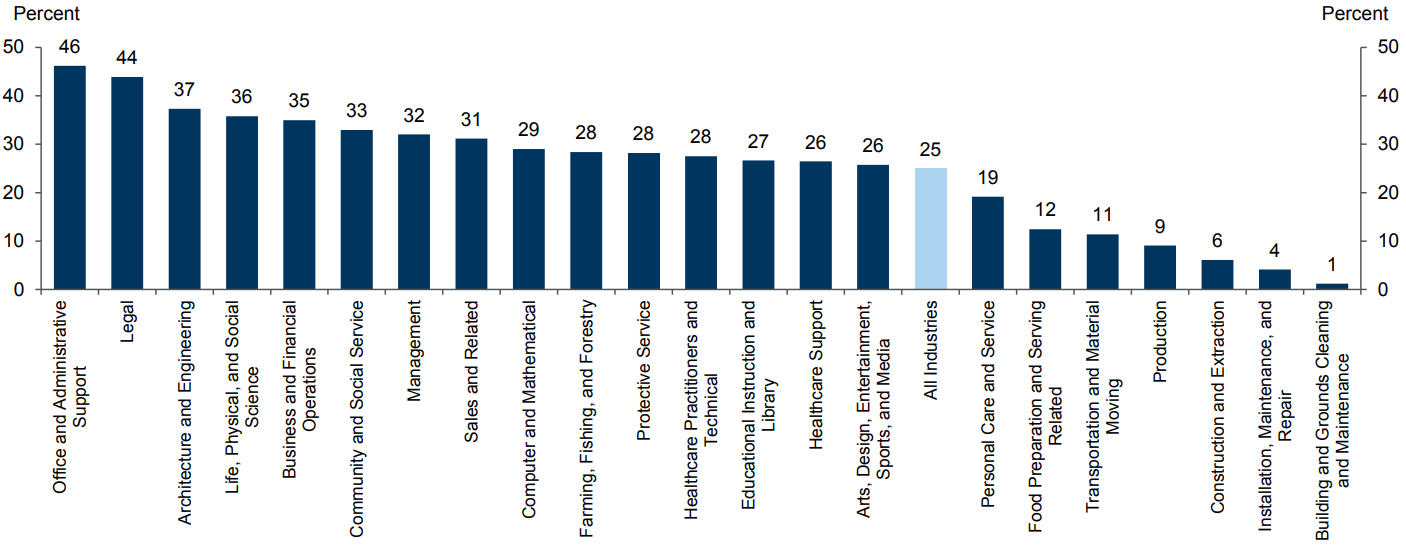
\includegraphics[width=\textwidth, height=.58\textheight]{../images/marcoref/share_of_industry_exposed_to_automation_ai.png}
        \caption{Porcentaje de la industria expuesta a la automatización por parte de la Inteligencia Artificial en Estados Unidos. Fuente: Goldman Sachs Global Investment Research (\citeyear{hatzius2023potentially}).}
        \label{fig:share_of_industry_exposed_to_automation_ai_gs}
    \end{figure}
    
    \begin{figure}
        \centering
        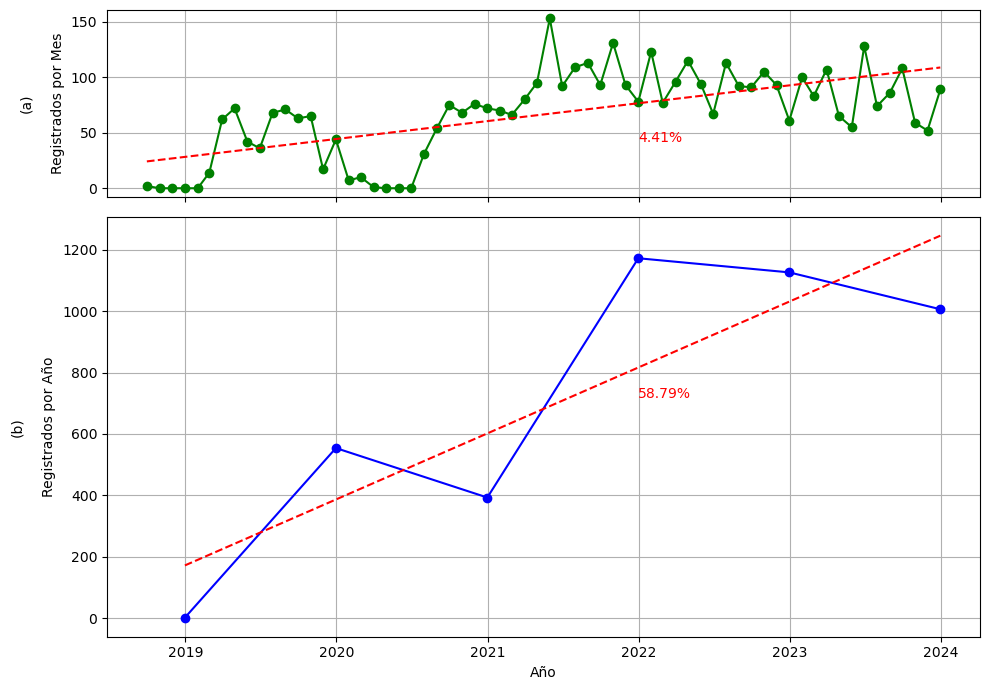
\includegraphics[width=\textwidth, height=.7\textheight]{../images/marcoref/tendencia_profesionales_syso_registrados.png}
        \caption{Registro de profesionales SySO:(a) Mensual (b) Anual.}
        \label{fig:profesionales_syso_registrados}
    \end{figure}

    \begin{figure}
      \centering
      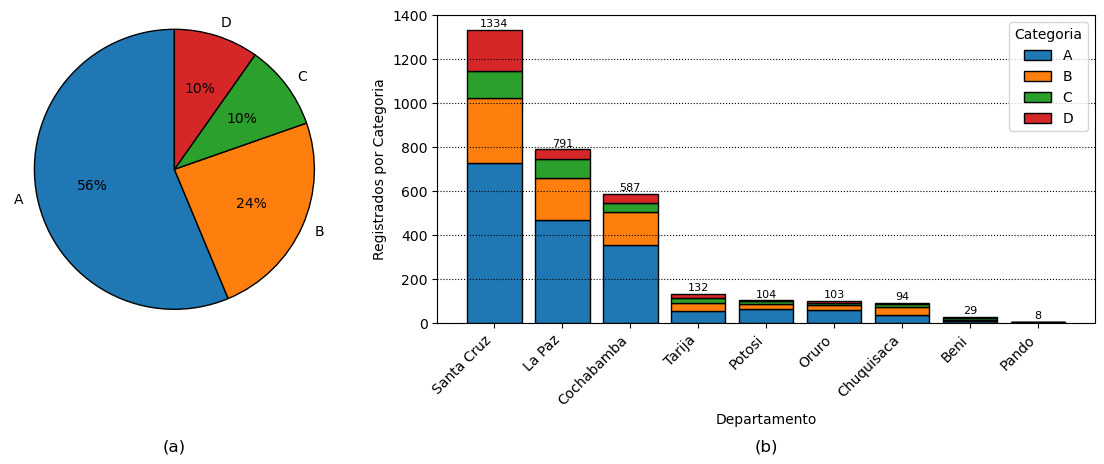
\includegraphics[width=1\textwidth]{../images/marcoref/profesionales_syso_por_categoria.png}
      \caption{Profesionales SST activos:\\Distribución de categorías (a) porcentual (b) por departamento.}
      \label{fig:profesionales_syso_por_categoria} 
    \end{figure}
\end{frame}

\begin{frame}{Definición del Problema}
  ¿Cómo impacta la falta de recursos humanos especializados en el cumplimiento de la NTS 009/23 por parte de las empresas en Bolivia?
\end{frame}

\begin{frame}[allowframebreaks]{Objetivos}
  \begin{block}{Objetivo general}
    Implementar un sistema automatizado basado en la NTS 009/23 que facilite la identificación de riesgos laborales, el desarrollo y la gestión eficaz de los PGSST.
  \end{block}
  \begin{block}{Objetivos específicos}
  \begin{itemize}
    \item Contextualizar la situación actual de los procesos para desarrollar los documentos requeridos por la NTS-009/23 mediante diagramas de flujo que reflejen las operaciones actuales.
    \item Determinar la arquitectura del sistema, incluyendo la estructura general, los componentes principales y las tecnologías a utilizar, para asegurar la escalabilidad, la modularidad y la eficiencia del sistema.
  \end{itemize}
  \end{block}

  \begin{itemize}
    \item Desarrollar las iteraciones del proyecto, estableciendo los objetivos específicos a alcanzar durante la fase de diseño, implementación y pruebas del sistema en cada iteración.
    \item Implementar el sistema utilizando la metodología de Desarrollo Guiado por Pruebas (TDD).
    \item Verificar la calidad del software tras cada iteración como parte del proceso de pruebas del sistema haciendo uso de la metodología Objetivo-Pregunta-Métrica (GQM) para asegurar la calidad en base al estándar ISO 25000:2014.
  \end{itemize}

\end{frame}

\begin{frame}{Justificación}
  \begin{block}{Justificación legal}
  La implementación del sistema se fundamenta en la NTS-009/23 y la Ley General de Higiene, Seguridad Ocupacional y Bienestar.
  \end{block}
  \begin{block}{Justificación tecnológica}
  La automatización y la IA ofrecen una oportunidad para mejorar la gestión de la seguridad y salud ocupacional.
  \end{block}
  \begin{block}{Justificación social}
  Mejorar las condiciones de trabajo beneficia a los trabajadores y a la sociedad en general.
  \end{block}
\end{frame}

\begin{frame}[allowframebreaks]{Delimitación}
  \begin{block}{Límites}
  \begin{itemize}
    \item Los documentos del software se ajustan a los requisitos técnicos de NTS-009/23.
    \item Contenido del software conforme a ISO 45001:2018 para seguridad y salud laboral.
    \item ISO 25000:2014 guía la evaluación del producto de software.
    \item La aplicación requiere conexión a internet para su uso.
    \item El software no contará con herramientas especializadas en la automatización de los estudios de higiene. Se limitará a plantillas para rellenar y automatizar el análisis de los datos recolectados por profesional habilitado.
  \end{itemize}
  \end{block}
  \framebreak
  \begin{block}{Alcances}
  \begin{itemize}
    \item Prototipo funcional de aplicación web que permita agilizar el proceso de desarrollo un de PGSST mediante generación automática de tres de los trece documentos solicitados por la NTS 009/23 de acuerdo a los requisitos recolectados de entrevistas a profesionales en el area.
    \item Entrevistas realizadas a los usuarios objetivo del producto.
    \item Documentación de la investigación de las tecnologías que se utilizarán para el
    desarrollo del software final.
    \item Documentación del desarrollo del software, en el cual se incluirá los detalles de la automatización del desarrollo de un PGSST y un manual de usuario.
  \end{itemize}
  \end{block}
\end{frame}

%--------------------------------------------------------------------------------
\section{Marco teórico y legal}

\begin{frame}{PGSST:Actividades}
  \begin{minipage}[t]{0.48\textwidth}
    \scriptsize
    \textbf{1.} Identificación de riesgos y evaluación de riesgos mediante la Matriz IPER.
    
    \textbf{2.} Estudios de Higiene.
    
    \textbf{3.} Descripción de la situación Actual e implementación de propuestas con respecto a:
    \begin{itemize}
      \item Orden y limpieza
      \item Infraestructura
      \item Instalaciones eléctricas
      \item Servicios higiénicos
      \item Vestuario y casilleros
      \item Equipos eléctricos
      \item Maquinaria, equipos y herramientas
      \item Almacenamiento, manipulación y transporte de sustancias peligrosas
      \item Gestión de residuos y señalización
      \item Ergonomía
    \end{itemize}
  \end{minipage}
  \hfill
  \begin{minipage}[t]{0.48\textwidth}
    \scriptsize
    
    \textbf{4.} Planificación de Capacitaciones Generales y Específicas con respecto a la Matriz de Identificación de Peligros y Evaluación de Riesgos (IPER).
    
    \textbf{5.} Organización y Conformación del Comité Mixto de Higiene y Salud Ocupacional.
    
    \textbf{6.} Elaboración del Plan de Emergencia:
    \begin{itemize}
      \item Procedimiento de Evacuación
      \item Procedimiento de Intervención
      \item Manual de Primeros Auxilios
    \end{itemize}
    
    \textbf{7.} Evaluación de Técnico Social.
  \end{minipage}
\end{frame}

\begin{frame}{PGSST:Organización Documental}
  \scriptsize
  \begin{enumerate}
    \item Política de seguridad
    \item Descripción de los procesos
    \item Matriz de Identificación de Peligros y Evaluación de Riesgos
    \item Estudios Monitoreos de Higiene
    \item Actividades de alto riesgo
    \item Descripción de las condiciones actuales
    \item Investigación de Accidentes
    \item Dotación de Ropa de Trabajo
    \item Inducción, Capacitación, concientización y comunicación
    \item Comité Mixto
    \item Inspección Internas en SST
    \item Plan de emergencia
    \item Medicina de Trabajo
\end{enumerate}
\end{frame}

\begin{frame}[allowframebreaks]{Legislación Aplicable a la SySO}
  \begin{itemize}
      \item Normativa obligatoria
      \begin{itemize}
          \item Constitución Política del Estado
          \item Ley General del Trabajo
          \item Reglamento de la Ley General de Trabajo
          \item Ley General de Higiene, Seguridad Ocupacional y Bienestar
          \item Disposiciones Complementarias\\ \quad Resolución Ministerial N° 992/23\\ \quad Resolución Ministerial N° 437/22\\ \quad Resolución Ministerial N° 849/14\\ \quad Resolución Ministerial N° 527/09
      \end{itemize}
      \framebreak
      \item Normativa voluntaria
      \begin{itemize}
          \item NB/ISO 62005:2005 - Calidad de Aire
          \item NB/ISO 55001:2005 - Señalización
          \item NB/ISO 51002:2012 - Iluminación
          \item NB/ISO 7243:2018 - Estrés térmico
          \item NB/ISO 45001:2018 - Sistema de Gestión Seguridad y Salud en el Trabajo
          \item NB/ISO 51001:2022 - Ventilación general de los lugares de trabajo
          \item NB/ISO 58005:2022 - Prevención y protección contra incendios
          \item NB/ISO 11226:2022 - Evaluación de posturas de trabajo estáticas
      \end{itemize}
  \end{itemize}
\end{frame}

\begin{frame}{Metodología de Desarrollo de Software}

  \begin{figure}
    \centering
    \resizebox{\textwidth}{!}{
    {\setlength{\fboxsep}{14pt} % Adjust the padding inside the \fbox
    \fbox{
        \begin{tikzpicture}[
            node distance= 5mm, 
            start chain = A going right, 
            block/.style = {rectangle, fill=blue!10, draw, minimum height=2em, text width=9em, align=center, on chain},
            arrow/.style = {-{Latex[width=8, length=6]},thick}]
            % nodes
            \begin{scope}[every node/.style={block}]
            \node {Requisitos};                  % A-1
            \node {Planificación};
            \node [xshift=15,yshift=77]{Inicio de la Iteración};
            \node [below=of A-3.south] {Diseño};
            \node [below=of A-4.south]{Implementación:TDD};
            \node [below=of A-5.south]{Pruebas del Sistema};
            \node [below=of A-6.south]{Retrospectiva};
            \end{scope}
            \node (iteration) [draw, very thin, inner ysep=10, inner xsep=10,  fit=(A-3) (A-7)] {};
            % Connections
            \draw [arrow] (A-1.east) -- (A-2.west);
            \draw [arrow] (A-2.east) -- (iteration.west);
            \draw [arrow] (A-3.south) -- (A-4.north);
            \draw [arrow] (A-4.south) -- (A-5.north);
            \draw [arrow] (A-5.south) -- (A-6.north);
            \draw [arrow] (A-6.south) -- (A-7.north);
            \draw [arrow, dashed] (A-7.east) -- ++(1,0) |- (A-3.east);
            \draw [arrow, dashed] (A-7.west) -| (A-2.south);
            \draw [arrow, dashed] (A-2.north) |- (A-3.west);
            % Text
            \node [below=of iteration.south] {Iteración de Desarrollo};
            \node (txt_func)[above=of A-1.north] {Funcionales};
            \node (txt_nfunc)[above=of txt_func.north, ,yshift=-8] {No funcionales};
        \end{tikzpicture}
        }
    }
}
      \caption{\footnotesize Proceso de desarrollo bajo la metodología PXP.}
      \scriptsize{{Elaboración propia a partir de ``\textit{\citefield{dzhurov2009personal}{title}}'' (\citeyear{dzhurov2009personal}).}}
    \label{fig:modelo_desarrollo_pxp} 
  \end{figure}

\end{frame}

\begin{frame}{Análisis y Evaluación de Software}
  \begin{table}[ht]
  \caption{Métodos y fases de evaluación de planificadas.}
  \label{tab:evaluacion_software}
  \centering
  \scriptsize
  \begin{tabularx}{\textwidth}{|l|X|X|}
  \hline
  \textbf{¿Qué?} & \textbf{¿Cómo?} & \textbf{¿Cuando?:Fase} \\
  \hline
  ISO 2500n & Define términos & Planificación y eval. \\
  \hline
  ISO 2501n & Define modelo de eval & Planificación \\
  \hline
  ISO 2502n & Métricas de calidad & Desarrollo y eval. final \\
  \hline
  ISO 2503n & Especifica req. de calidad & Planificación \\
  \hline
  ISO 2504n & Guías para evaluar la calidad & Eval. final \\
  \hline
  GQM & Define objetivos, preguntas y métricas & Planificación y eval. final \\
  \hline
  P. Unitarias & Pruebas modulares & Cada iteración de desarrollo \\
  \hline
  P. de Integración & Verificar integración & Al finalizar cada iteración \\
  \hline
  P. de Regresión & Evitar que nuevas modificaciones afecten el código & Después de cada iteración \\
  \hline
  P. de Sistema & Eval. completa del sistema & Al finalizar las iteraciones \\
  \hline
  P. de Desempeño & Med. eficiencia y rendimiento & Cierre y eval. final \\
  \hline
  P. de Carga & Eval. desempeño bajo cargas esperada & Cierre y eval. final \\
  \hline
  P.s de Estrés & Determinar lím. del sistema & Cierre y eval. final \\
  \hline
  P. con Usuarios & Pruebas en campo & Cierre y eval. final \\
  \hline
  \end{tabularx}
\end{table} 
\end{frame}

\begin{frame}[allowframebreaks]{Analisis de Competidores}

  \begin{figure}[htb]
    \centering
    \fbox{
        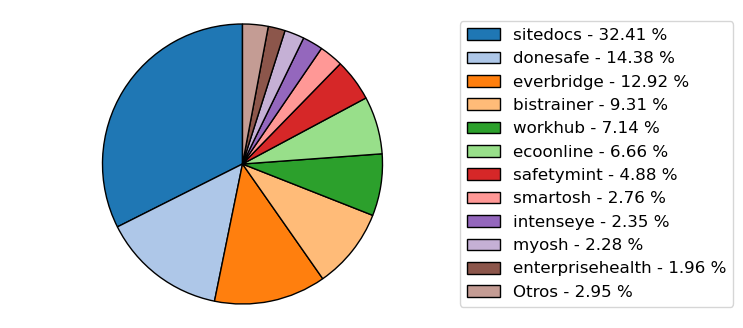
\includegraphics[width=0.95\linewidth]
        {../images/marcopractico/planificacion/visitas_por_dominio.png}
    }
    \caption{\footnotesize Participación de Mercado de los Principales Competidores}
    \footnotesize{{Elaboración propia a partir de datos obtenidos por medio de ``\textit{SEMrush ME}''.}}
    \label{fig:visitas_por_dominio}
  \end{figure}

  \begin{figure}[htb]
    \centering
    \fbox{
        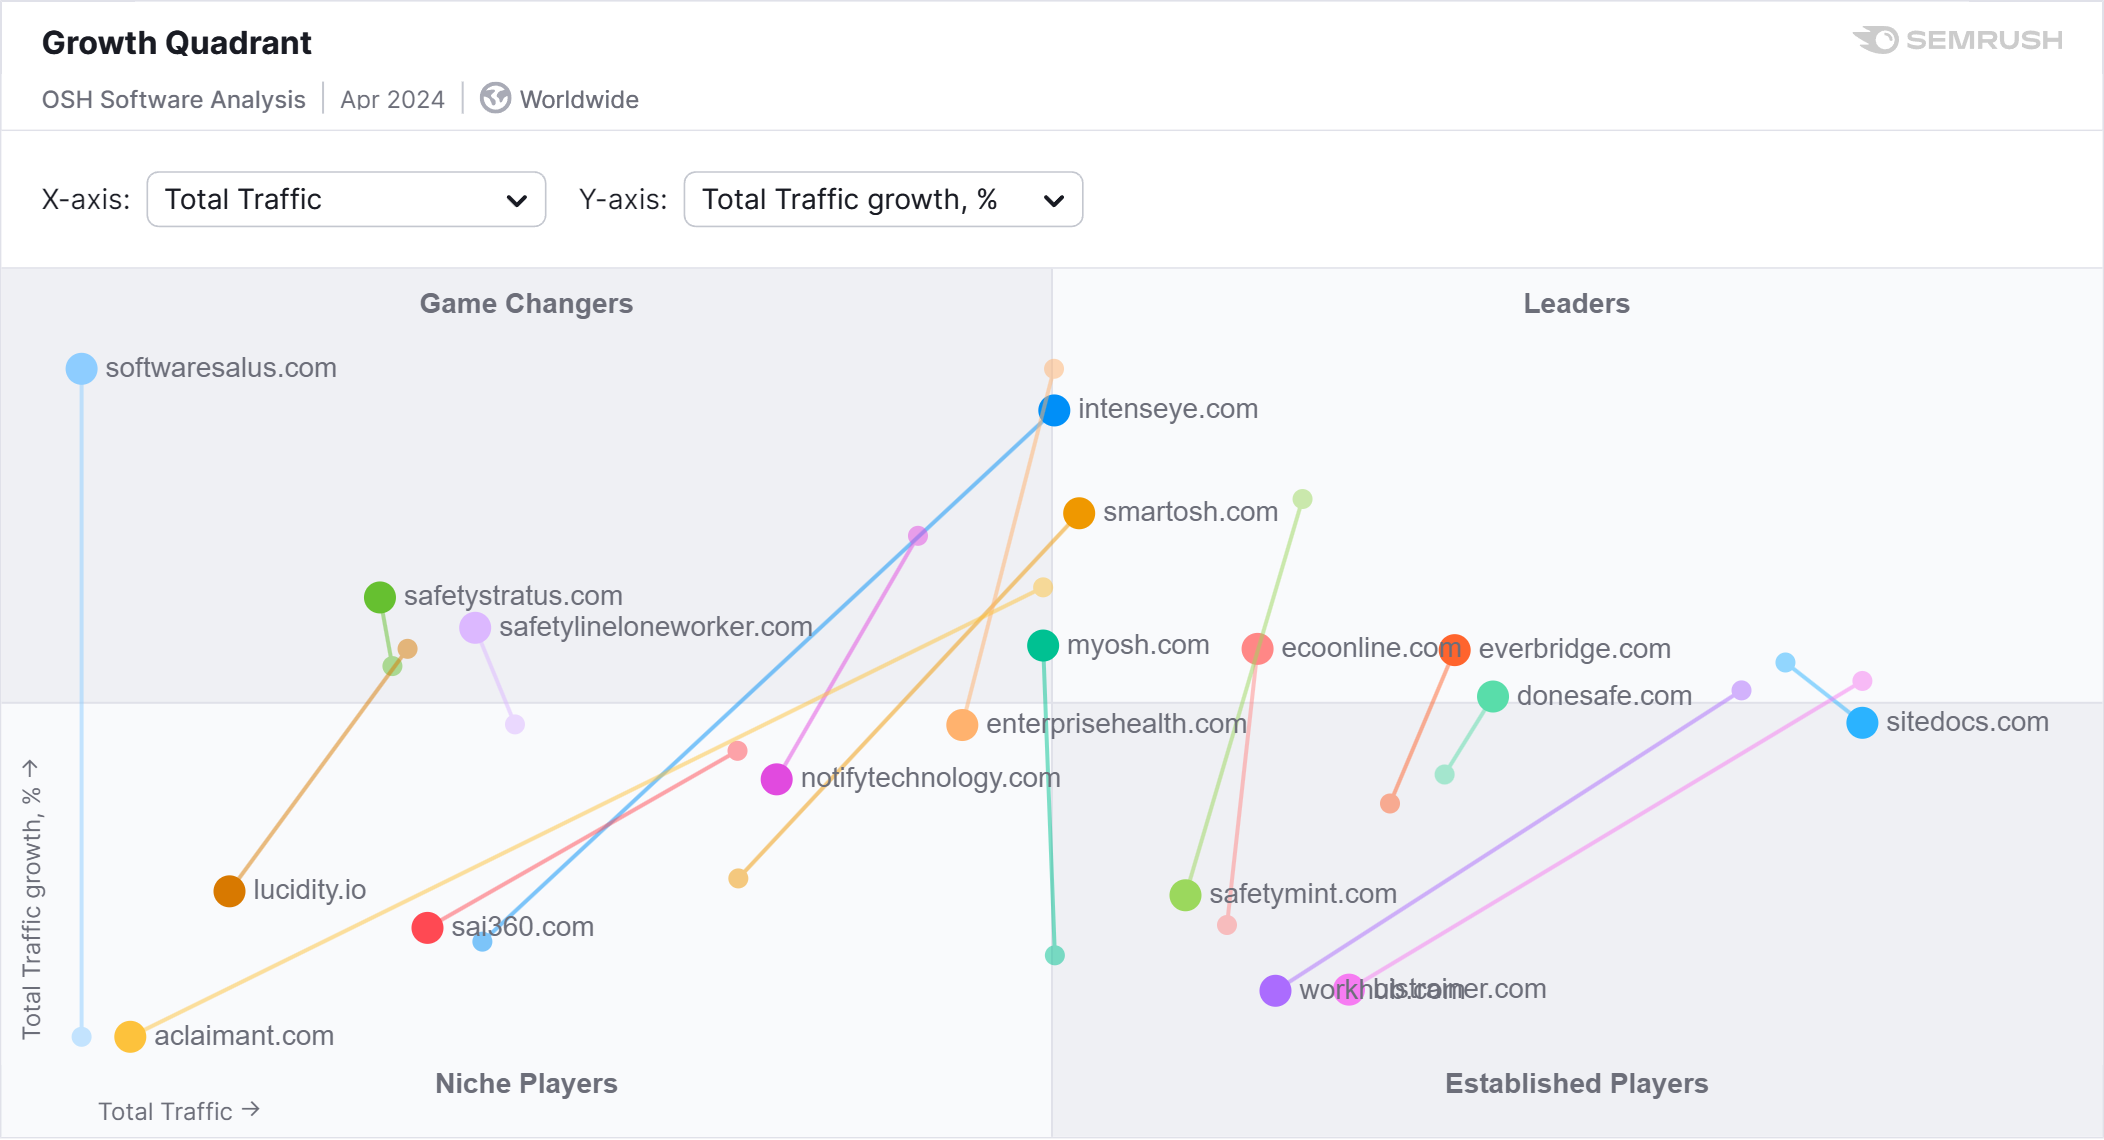
\includegraphics[width=0.95\linewidth]
        {../images/marcopractico/planificacion/GrowthQuadrant.png}
    }
    \caption{Matriz de Competidores: \textit{OSH Software}}
	  \footnotesize{Fuente: Elaborado por ``\textit{SEMrush ME}''.}
    \label{fig:MatrizCompetidores}
  \end{figure}

\end{frame}

\begin{frame}{Analisis de Costos}

  \begin{table}[ht]
    \footnotesize
    \centering
    \caption{Inversión Total Inicial MVP}
    \label{tab:inversion_total}
    \begin{tabularx}{\textwidth}{|X|r|}
        \hline
        \textbf{Concepto} & \textbf{Costo (Bs)} \\
        \hline
        Costo de Desarrollo & 52,560.00 \\
        Costos de Infraestructura & 2,224.06 \\
        Gastos Legales & 4,997.00 \\
        \hline
        \textbf{Total} & \textbf{59,781.06} \\
        \hline
    \end{tabularx}
  \end{table}

  \begin{table}[htb]
    \footnotesize
    \centering
    \caption{Proyección financiera del proyecto completo bajo el modelo SaaS}
    \label{tab:proyeccion_financiera}
    \begin{tabularx}{\textwidth}{|c|r|>{\raggedleft\arraybackslash}X|>{\raggedleft\arraybackslash}X|>{\raggedleft\arraybackslash}X|r|}
        \hline
        \thead{Año} & \thead{Usuarios\\Mensuales} & \thead{Gastos\\Anuales (Bs)}  & \thead{Ingresos\\Anuales (Bs)}  & \thead{Balance\\Anual (Bs)} & \thead{C/B} \\ \hline
        0 & 0 & 276,755.53 & 00.00 & -276,755.53 & 0.00 \\ \hline
        1 & 330 & 98,688.72 & 277,200.00 & 178,511.28 & 2.81 \\ \hline
        2 & 525 & 98,688.72 & 441,000.00 & 342,311.28 & 4.47 \\ \hline
        3 & 834 & 98,688.72 & 700,560.00 & 601,871.28 & 7.10 \\ \hline
        4 & 1325 & 98,688.72 & 1,113,000.00 & 1,014,311.28 & 11.28 \\ \hline
        5 & 2104 & 98,688.72 & 1,767,360.00 & 1,668,671.28 & 17.91 \\ \hline
    \end{tabularx}
  \end{table} 

\end{frame}

\begin{frame}{Cronograma del Proyecto}

  {\small \begin{table}[htb]
    \caption{Cronograma del proyecto.}
    \label{tab:cronograma_proyecto}
    \centering
    \resizebox{\textwidth}{!}{%
    \begin{tabular}{|c|c|c|c|c|}
        \hline
        \rowcolor{lightgray} \textbf{Etapa} & \textbf{Tareas} & \textbf{Fecha de Inicio} & \textbf{Fecha de Fin} & \textbf{Dias} \\
        \hline 
        \rowcolor{lightgray} Def. Requisitos &  & 01/02/2024 & 10/05/2024 & 99 \\ \hline
        ~ & Entrega Marco Referencial & \multicolumn{2}{|c|}{15/03/2024} & 1 \\ \hline
        ~ & Entrega de avance & \multicolumn{2}{|c|}{03/05/2024} & 1 \\ \hline
        ~ & Defensa & \multicolumn{2}{|c|}{10/05/2024} & 1 \\ \hline
        \rowcolor{lightgray} Planificación &  & 15/03/2024 & 30/06/2024 & 107 \\ \hline
        ~ & Entrega de avance & \multicolumn{2}{|c|}{24/05/2024} & 1 \\ \hline
        ~ & Entrega de perfil & \multicolumn{2}{|c|}{07/06/2024} & 1 \\ \hline
        ~ & Defensa & \multicolumn{2}{|c|}{14/06/2024} & 1 \\ \hline
        ~ & Análisis de Procesos & 17/06/2024 & 23/06/2024 & 6 \\ \hline
        ~ & Diseño de Arq. & 24/06/2024 & 30/06/2024 & 6 \\ \hline
        \rowcolor{lightgray} Desarrollo &  & 01/07/2024 & 01/09/2024 & 62 \\ \hline
        ~ & Iteración 1 & 01/07/2024 & 21/07/2024 & 20 \\ \hline
        ~ & Iteración 2 & 22/07/2024 & 11/08/2024 & 20 \\ \hline
        ~ & Iteración 3 & 12/08/2024 & 01/09/2024 & 20 \\ \hline
        \rowcolor{lightgray} Cierre &  & 02/09/2024 & 29/09/2024 & 27 \\ \hline
        ~ & Preparación de Documentación  & 02/09/2024 & 08/09/2024 & 6 \\ \hline
        ~ & Capacitación de Usuarios & 09/09/2024 & 15/09/2024 & 6 \\ \hline
        ~ & Monitoreo Inicial y Ajustes & 16/09/2024 & 22/09/2024 & 6 \\ \hline
        ~ & Pruebas con Usuarios & 23/09/2024 & 29/09/2024 & 6 \\
        \hline
    \end{tabular}
    }
\end{table}}

\end{frame}

\end{document}